% !TeX spellcheck = en_US
% !TeX encoding = UTF-8
% !TeX root = ../document.tex

\chapter{Model Unspecific Search}

\section{Motivation}
A collision at an energy of \SI{13}{\TeV} can create a large amount of different particles. Solely by combinatorics, it follows that a lot of different final states are accessible.

Most dedicated searches tend to focus on one or a few final states that represent the signature of the theory under investigation. This leaves many final states not examined, either because of the complexity of the final state or because there is no analysis group currently working on a corresponding theory.

One of the goals of the model unspecific search is to gain knowledge from these additional final states. Additionally, the model unspecific search aims to obtain a global interpretation of the agreement between simulation and observed data across a broad range of final states.

\section{Previous Works}
The approach of a model unspecific search is not a new concept: In 1998, a note about an unspecific search has been written at the L3 experiment (\ac{LEP})\cite{Hebbeker:GlobalComparisonL3}, and in 2004, a similar approach has been applied to data of the D0-experiment at the Tevatron proton-antiproton collider at Fermilab\cite{Biallass:ModelIndependentSearch}.

At \ac{CMS}, the analysis has been developed and regularly applied to observed data since 2009\cite{Schmitz:ModelUnspecificSearch,Hof:ImplementationModelIndependent,Dietz-Laursonn:ModelUnspecificSearch,Olschewski:StudyAlternativeStatistical,Brodski:ModelUnspecificSearch,Pieta:MUSiCModelUnspecific,Papacz:ModelUnspecificSearch,Albert:ExtensionModelUnspecific,Roemer:ModelUnspecificSearch,CMS:CMS-PAS-EXO-14-016,Knutzen:softwarereinterpretationmodel,Durchardt:MUSiCModelUnspecific}. 
This thesis bases on the most recent implementation of the \ac{MUSiC} analysis.\todo{ok so?}

Very recently, the \ac{ATLAS} collaboration published a conference note analyzing \SI{3.2}{\per\femto\barn} of \ac{LHC} data at $\sqrt{s} = \SI{13}{\TeV}$ using a similar model-independent search \cite{ATLAS:ATLAS-CONF-2017-001}. 

\section{Procedure}
The input to the \ac{MUSiC} analysis are reconstructed events of observed as well as simulated data, which have been centrally reconstructed by the \ac{CMS} collaboration.
As first step of the \ac{MUSiC} analysis, requirements on events and physics objects are applied, discarding unwanted events and extracting objects for the \ac{MUSiC} analysis (see \fref{chap:selection}).
Afterwards, each event is classified sorted into so-called \emph{event classes}, sets of events that share the same final state.
For each event class, the kinematic variables of each event are calculated and \emph{kinematic distributions} are aggregated.
Up to this point, the same procedure is applied to simulated data and observed data.
Subsequently, an automated search algorithms finds the largest deviation between data and simulation within each kinematic distribution of each event class. Afterwards, the global significance of each deviation is estimated from Standard-Model only simulations.

\section{Event Classes}
An event class is a set of events sharing the same final state. The final state is indicated by the name of the event class: All events in the class named \eventclass{2\Pe + 1\Pmu}, for example, contain two electrons and one muon in the final state.

There are three types of event classes: \emph{exclusive}, \emph{inclusive} and \emph{jet inclusive}.

Events in the exclusive event classes contain exactly the indicated (and no additional) particles in their final state. Each event thus belongs to exactly one exclusive event class.

Inclusive event classes are denoted with the suffix "\eventclass{+ X}" in the name (for example \eventclass{2\Pe + 1\Pmu + X}). Their final state contains the explicitly stated particles plus any additional ones. Each event can be assigned any number of inclusive event classes. One advantage of this procedure is a larger number of events per class which can be beneficial \todo{for what?}. However, the correct combination of statistical results across multiple inclusive event classes is not trivial.

Jet inclusive event classes are denoted with the suffix "\eventclass{+ Njets}" in the event class name (e.g. \eventclass{2 \Pe + 1\Pmu + Njets}). Events contained in a jet inclusive event class may contain any number of jets in addition to the explicitly stated objects. This increases the number of events per class, as effects like initial or final state radiation are ignored, leading to reduced statistical uncertainties.

In any case, the kinematic variables are only calculated from the objects explicitly stated in the class name, in our example two electrons and one muon.


\section{Particle Types}
Not all particle types that can be identified by the experiment are used within the classification. Instead, \ac{MUSiC} focuses on a set of five particle types which can be measured most precisely.
Additionally, certain selection criteria are imposed onto each particle in the final state to obtain an unambiguous final state.
The particle types and identification criteria are described in the following sections.

big picture
why ids (why not just reco)
general id criteria: pt, tracks, shower


\subsection{Electrons}



\subsection{Muons}

\subsection{Photons}

\subsection{Jets}

\subsection{Missing Transverse Energy}

\subsection{Possible Extensions}
The analysis can be extended to identify more particle types by their decay products, called \emph{tagging}. Possible tagging choices are \Pqb-tagging, \Ptau-tagging or \PZ-tagging.
This thesis will investigate the increase of sensitivity using \Pqb-tagging. The method is further described in chapter \todo{ref}.

\section{Transverse Momentum and Transverse Energy}
\todo{context?}

Interaction cross sections are often dependent on the amount of momentum involved. In t-channel diagrams, the entire momentum transfer can be measured by calculating the combined invariant mass of decay products.
In order to achieve this goal, one must know all four components of the momentum of all created particles. If the final state contains neutrinos, which are not detectable by the detector, this is not achievable.

In other experiments like \ac{LEP}, one could use conservation of momentum and the known momentum of colliding particles to reconstruct the neutrino four-momentum and the momentum transfer. At the \ac{LHC} this is also impossible: The total proton momentum is distributed unevenly between the constituent quarks and gluons and thus the momentum involved in a collision is only known up to statistical probability.

The mitigation pursued at \ac{CMS} is to only regard kinematics in the transverse plane, orthogonally to the beam pipe. Projection of the kinematic (three-)momentum onto the transverse plane gives the so-called \emph{transverse momentum} \pT.

An additional property of the transverse momentum is that it can be directly observed: Since the magnetic field lines are parallel to the beam direction, the Lorentz force only acts in the transverse plane, allowing direct observation of the transverse momentum.

Assuming $p_x$, $p_y$, $E$ and $m$ can be observed directly (e.g. via track curvature) or indirectly (e.g. via particle identification), we can define the transverse momentum and transverse energy as follows:
\begin{align*}
\vec{p}_T &\defeq \left( p_x, p_y, 0 \right)^T  \\
\vec{E}_T &\defeq E \frac{\vec{p}_T}{\abs{\vec{p}}} = \frac{\vec{p}_T}{\sqrt{1-\left(m/E\right)^2}}
\end{align*}

Note that in the approximation of massless ($m \approx 0$) particles: $\vec{p}_T = \vec{E}_T$. % $ = \vec{M}_T$.

%cross sections are dependent of momentum transfer
%in t-channel diagrams: momentum transfer is invariant mass of created particles
%calculate inv mass from 4-vectors of all particles
%problem if neutrinos are produced
%other approaches (both done at LEP): control COM energy of interaction precisely, or use momentum conservation to reconstruct neutrino 4-momentum
%problem: energy of and initial momentum in beam direction unknown because of partons
%mitigation: use knowledge about momentum in transverse plane, calculate momenta and energy there
%pT has additional advantages: measured directly (magnetic field) and is invariant regarding pdfs/z-boosts

\section{Kinematic Variables and Distributions}
For each event, the \ac{MUSiC} classification calculates three scalar variables: the sum of transverse momenta, the invariant mass and the missing transverse energy.

The sum of transverse momenta is the most directly observed variable. For charged particles, the transverse momentum can be deduced directly from the curvature within the magnetic field. The transverse momentum is invariant against Lorentz-boosts in the $z$-direction from the uneven momentum distribution within the proton.
In the following, the sum of transverse momenta will be denoted with \sumpT and defined as follows:
\begin{equation}
    \sumpT \defeq \sum_i \abs{\vec{p}_{T,i}} 
\end{equation}

The invariant mass is, as mentioned before, very sensitive to resonances in the t-channel. If the event class definition contains missing transversal energy passing the selection criteria, the invariant mass will not be computed, instead the transversal mass is used. The variables are denoted with \Minv and \MT respectively and defined as:
\begin{align}
    \Minv &\defeq \sqrt{\left(\sum_i E_i\right)^2 - \left(\sum_i \vec{p}_i\right)^2} \\
    \MT &\defeq \sqrt{\left(\sum_i E_{T,i}\right)^2 - \left(\sum_i \vec{p}_{T,i}\right)^2}     
\end{align}

The third kinematic variable is missing transversal energy. This variable is only calculated if the event class definition explicitly contains missing transversal energy.
The variable is denoted with \MET defined as follows:
\begin{equation}
    \MET \defeq \abs{- \sum_i \vec{E}_{T,i}} 
\end{equation}


\section{Search for Deviations}
\label{sec:deviations_search}

\newcommand{\TS}{\ensuremath{\uptheta}\xspace}
\newcommand{\TSmin}{\ensuremath{\uptheta_\text{min}}\xspace}

After the classification follows an automated search for deviations. The search is performed on each distribution of each event class separately as follows:
First, multiple bins are combined to a \emph{region}, according to the rules in the following section. Then, a test statistic \TS for each region is calculated. The region with the lowest value of \TS, called \TSmin, is selected. This region will be called \acfi{RoI}. 
Subsequently, a global $\ptilde$-value for the region is calculated. This $\ptilde$-value expresses the probability of finding a deviation with $\TS \leq \TSmin$ purely by chance. Details on the procedure can be found in \fref{sec:global_significance}.

\subsection{Search Space}
The search is performed on so-called regions. A region is a set of adjacent bins and is represented by the combined number of expected and observed events as well as a combined uncertainty.

For the \sumpT and \MET kinematic distributions, the minimal number of bins in a region is \num{3}, in order to be insensitive towards narrow deviations from \ac{MC} statistics \todo{explain spikes}.
For a increased sensitivity to resonant deviations, the minimal number of bins in the \Minv and \MT distributions is \num{1}.

An additional criterion on the regions is based on the number of simulated events in a region. If a region shows a lack of simulated events, the test statistic is not computed for this particular region. Since each region (that is not the entire distribution) is embedded in a larger region, regions skipped in this step are still considered. \todo{low stats ausfuerlicher erklaeren?}

The combined number of events and the combined uncertainty for each region is calculated as
\begin{align}
     N_{\text{total},\text{exp}} &= \sum_i N_{i, \text{exp}} \\   
     N_{\text{total},\text{obs}} &= \sum_i N_{i, \text{obs}} \\
     \sigma_\text{total} &= \sqrt{\sum_i \sigma_i^2 + 2 \sum_{i,j} \rho_{i,j}\sigma_i\sigma_j}
\end{align}
where $\rho_{i,j}$ is the correlation coefficient for the uncertainty $\sigma$ between the bins $i$ and $j$.

Some uncertainties, such as the statistical uncertainty on the simulated number of events, are completely uncorrelated between the bins. The correlation coefficient thus is $\rho_{i,j} = 0$ and the total uncertainty is the quadratic sum of the bin uncertainties.

Other uncertainties are correlated between bins. An example for this is the uncertainty on the luminosity measurement, which affects all bins of all distributions the same way. We treat any uncertainty that is assumed to be correlated to some extend as fully correlated ($\rho_{i,j} = 1$) and calculate the combined uncertainty as linear sum. This method possibly overestimates the total uncertainty, in case the correlation coefficient is somewhere between 0 and 1, leading to a lower \todo{(conservative?)} sensitivity.

\subsection{Global Significance}
\label{sec:global_significance}

The goal of the automated search is to find the largest deviation between expected and observed number of events in a region. The size of a deviation is expressed as value of the test statistic \TS. A larger deviation will result in a smaller value of \TS.
The formula for computing \TS will be derived in the next chapter. \todo{mention \TS = local p value?}

From the test statistic, we will calculate a global significance, to which we refer as \ptilde. It expresses the probability of finding a deviation equally large or larger than the observed one somewhere in the distribution if the expectation were true.

The simplest way of calculating \ptilde would be to first calculate a local $p$-value from the test statistic and then apply a correction factor to it. A suitable correction factor could be estimated using combinatorics if the possible values of the local $p$-value were uncorrelated. This method is also called \emph{Bonferroni correction}. 

In our case, a purely analytically calculation is not possible because the connected bin regions overlap and thus the local significances are correlated.

Instead, we use a simulation-based approach:
We simulate possible experimental outcomes based on the distribution of expected number of events, and refer to each simulation round as \emph{pseudo-experiment}.
During each pseudo-experiment, we randomly draw a substitute observed distribution from the expected number of events. 



correlated uncerts: shared value of standard gaussian multiplied with local width of uncert
uncorrelated: random from normal distribution
summed up
poissonian draw for quantum-phenomena

\begin{algorithm}
    \caption{Pseudo Experiment}
    \newcommand{\Nobs}{n}
    \newcommand{\Nexp}{N}
    \newcommand{\corr}{corr}    
    \newcommand{\uncorr}{uncorr}
    \newcommand{\x}{x}
        
    \begin{algorithmic}
        \Require $\Nexp_{i=1..n} \gets $ number of events in each bin $i$
        \Require $\corr_{i=1..n,j=0..c} \gets $ correlated uncertainty $j$ in each bin $i$
        \Require $\uncorr_{i=1..n,k=0..u} \gets $ uncorrelated uncertainty $j$ in each bin $i$
        
        \Statex
        
        \ForAll {correlated uncertainty $j$ in distribution}
            \State $\x_j \gets \text{RandNormal}(\mu = 0, \sigma = 1)$
        \EndFor
        
        \ForAll {bin $i$ in distribution}
            \State $\Nobs_i \gets \Nexp_i$
            \ForAll {correlated uncertainty $j$ in bin $i$}
                \State $\Nobs_i \gets \Nobs_i + \x_j \cdot \corr_{i,j}$
            \EndFor
            \ForAll {uncorrelated uncertainty $k$ in bin $i$}
                \State $\Nobs_i \gets \Nobs_i + \text{RandNormal}(\mu = 0, \sigma = \uncorr_{i,k})$
            \EndFor
            \State $\Nobs_i \gets \text{RandPoisson}(\Nobs_i)$
        \EndFor
    \end{algorithmic}
\end{algorithm}

The recipe for each pseudo-experiment is as follows:

Let $\sigma_u(i,j)$ be the value of the uncorrelated uncertainty and $\sigma_v(i,j)$ the value of a correlated uncertainty with index $j$ in bin $i$. Further, let $\ev{N_{i}}$ be the expected number of events in bin $i$.



Start by simulating a pseudo-true value for correlated uncertainties since this impacts all bins differently, we choose from a standard normal distribution $\mathcal{N}$:
\begin{equation}
    v_j \sim \mathcal{N}(\mu = 0, \sigma = 1)
\end{equation}

The impact factor for uncorrelated uncertainties is calculated separately for each bin:
\begin{equation}
    u_{i,j} \sim \mathcal{N}(\mu = 0, \sigma = 1) 
\end{equation}

\begin{equation}
    \ev{n_i} = \ev{N_i} + \sum_j^{\text{uncorrelated}} u_{i,k} \sigma_u(i,j) + \sum_k^{\text{correlated}} v_{i,k} \sigma_v(i,k)
\end{equation}

Finally draw an integer value from the Poisson distribution $\mathcal{P}$ with the expectation value $\ev{n_i}$.
\begin{equation}
    n_\text{obs} \sim \mathcal{P}(\lambda = \ev{n_i})
\end{equation}


For each \emph{pseudo-experiment}, we draw a random number of events for each bin of the distribution simultaneously. The number is drawn from the probability distribution caused by systematical and statistical uncertainty around \ac{SM} expectation value. 


 of \emph{pseudo-experiments}: For each bin of the distribution, a random number is drawn from the probability distribution caused by systematical and statistical uncertainty on the \ac{SM} expectation value. The resulting \emph{pseudo-distribution} is subsequently again compared to the expectation using the described search algorithm, yielding a local significance value \TS for each pseudo-experiment.
The step of randomly generating a distribution and searching for a deviation is repeated \num{e5} to \num{e6} \todo{number} times.

Finally, the global \ptilde-value is calculated by determining the rate of pseudo-experiments where $\TS_{\text{random}, \text{min}} < \TS_{\text{obs}, \text{min}}$. Note that the definition of a $p$-value ("probability to find a deviation equally large or larger as the observed one by chance") corresponds directly to the computed \ptilde-value in the frequentist interpretation.

%Within the (statistical and systematical) uncertainty distribution of the Standard Model  
%The statistical nature of the Standard-Model is simulated by randomly choosing values for the observed number of events in each bin.
%The probabilities of observing deviations are correlated between overlapping regions. 
%Since the regions' overlap, the regions are correlated. Thus, the probabilities of observing deviations by chance are correlated between overlapping regions.
%assess the significance of a deviation, expressed as probability to observe a deviation the same as or more extreme just by chance (given SM) SOMEWHERE in the distribution
%procedure also known as Bonferroni correction
%correction factor cannot be calculated analytically because of correlations between regions
%idea: pseudo-experiment, simulate circumstances using SM only, count more-extreme values, interpret fraction as probability (frequentist  approach)
%problem: need measure for "extremity" of deviation (-> also used for finding RoI)

\subsection{Test Statistic}
\label{sec:test_statistic}

measure "extremity" of deviation (-> for finding RoI as well as global correction)

choice is ambiguous

choice: value interpretable as probability for local deviation

back to definition: sum of probabilities of more extreme events

start using Poissonian probability
include Gaussian prior: either normal or log normal


most of the systematic uncertainties scale number of events in a region rather than a constant shift. examples: lumi, xsec, PDF, ID efficiency, misID


The total number of events is thus scaled by an unknown factor $X$, which is a random variable that emerges as product of multiple other random variables $x_i$.
In the following section, we will derive how $X$ is distributed.

We begin with rewriting the product in terms of a sum within an exponential distribution:
\begin{equation}
    X = \prod_i x_i = \prod_i \exp(\ln(x_i)) = \exp(\sum_i \ln(x_i))
\end{equation}
$\ln(x_i)$ is a random variable, and the central limit theorem implies that the sum is distributed according to the normal distribution.
\begin{equation}
    Y \defeq \sum_i \ln(x_i) \Rightarrow X = \exp(Y) \text{ and } f_Y(y) = \frac{1}{\sqrt{2\pi}\sigma} \exp(-\frac{1}{2}\left(\frac{y-\mu}{\sigma}\right)^2)
\end{equation}
After defining $Y$ as the normally distributed variable with the probability density $f_Y(y)$, we introduce a new unknown probability density function $g_X(x)$:
\begin{equation}
    f_Y(y) \: \dd y \eqdef g_X(x) \: \dd x 
\end{equation}
Finally, we can insert all definitions, calculate the derivative and write the distribution function dependent of $x$:
\begin{align}
    g_X(x) &= f_Y(y) \: \dv{y}{x} \\
    &= f_Y(\ln{x}) \: \dv{\ln{x}}{x} \\
    &= f_Y(\ln{x}) \: \frac{1}{\abs{x}} \\
    &= \frac{1}{\sqrt{2\pi}\sigma\abs{x}} \exp(-\frac{1}{2}\left(\frac{\ln{x}-\mu}{\sigma}\right)^2)
\end{align}
The result is known as \emph{log-normal distribution} and is the probability density function of a product of random variables.

By performing two substitutions, we obtain a parametrization with a more meaningful interpretation:
\begin{equation}
    \sigma \rightarrow \ln{k} \text{ and } \mu \rightarrow \ln{x_0}
    \label{eq:log_normal_substitution}
\end{equation}
\begin{equation}
    g_X(x) = \frac{1}{\sqrt{2\pi}\abs{x}\ln{k}} \exp(-\frac{1}{2}\left(\frac{\ln(x/x_0)}{\ln{k}}\right)^2)
\end{equation}

\todo{explain meaning of parameters}

\subsection{Treatment of Regions With Too Few Simulated Events}


\subsection{Look-Elsewhere-Effects}
\subsubsection{Regions}
corrected using global significance 

\subsubsection{Classes}
\subsubsection{Distributions}

\section{Implementation}
\subsection{Software Environment}
CMSSW, ROOT, Python/C++

\subsection{Analysis Framework}
Skimming, Pxl, TAPAS, MUSiC

\subsection{MUSiC Workflow}

\subsection{Lookup-Table}
During the automated search algorithm, most of the computation time is spent calculating \TS according to \todo{ref?}, which involves integration and summation over a large number of terms.

To decrease the amount of time spent in this step, we implemented a three dimensional \acfi{LUT}. The table consists of \TS values for the most frequently used input parameters, such that the expensive runtime computation is replaced by retrieving a precomputed value from a static block of memory.

The \acf{LUT} is generated as a separate file during compilation and is about \SI{80}{\mega\byte} in size.

\subsubsection{Implementation}
The precise lookup procedure for $\TS_\text{LUT}(N_\text{obs}, N_\text{MC}, \sigma)$ \todo{parameter names and order?)} is as follows:
\begin{enumerate}
    \item Determine real-valued indices $i, j, k$ from the parameter values $N_\text{obs}, N_\text{MC}, \sigma$
    \item Check whether the calculated indices are valid, e.g. within table bounds
    \item Fetch four adjacent values from memory: $N_\text{obs}$ entry at $\floor i$, $N_\text{MC}$ and $\sigma$ entries at $\floor j, \ceil j, \floor k, \ceil k$.
    \item Use two dimensional linear interpolation in the $j, k$ plane to get a better estimate for \TS:
    \begin{align*}
        \TS_\text{LUT}(i, j, k) \approx \; &\TS(\floor i, \floor j, \floor k)(\ceil j - j)(\ceil k - k) \\
        + \; &\TS(\floor i, \ceil j, \floor k) (j - \floor j)(\ceil k - k) \\
        + \; &\TS(\floor i, \floor j, \ceil k) (\ceil j - j)(k - \floor k) \\
        + \; &\TS(\floor i, \ceil j, \ceil k) (j - \floor j)(k - \floor k)
    \end{align*}
    Note that $j - \floor j = 1 - (\ceil j - j)$.
    \item Discard the result if it is too small (less than $0.005$)
\end{enumerate}

If the value has not been found in the \ac{LUT}, either because of the table bounds or an otherwise untrusted value, the implementation falls back to the full expensive calculation of \TS.
Thus, the efficiency of the \ac{LUT} is determined by the probability that a requested value is contained in the table.

In order to improve accuracy around the most commonly used parameters ($N_\text{obs} = N_\text{exp}$, $N_\text{obs}$ small), the \ac{LUT} is organized in three regions, as illustrated in \fref{fig:lut_points}. In the so-called "grid region", the point spacing for the expected number of events is independent if the observed number of events. This results in a rectangular grid up to an observed yield of \num{10} and an expected yield of \num{20}.
The second, so-called "linear region" stretches up to an observed yield of \num{100}. In this region, every integer observed value corresponds to exactly one index, $i = N_\text{obs}$. Lastly, there is an exponential region, in which the spacing of observed points gradually becomes less dense, keeping the relative spacing constant.
In the dimension of the expected number of events, the \ac{LUT} is more densely spaced around $N_\text{exp} = N_\text{obs}$, because this is statistically the most common scenario. There is an exponential falloff in density which in theory expands from $N_\text{exp} = \num{0.1} N_\text{obs}$ up to $\num{5.0} N_\text{obs}$, very distant values, however, are vetoed by the $\TS_\text{LUT} > \num{0.005}$ threshold. In the third dimension, uncertainty, the grid is exponentially spaced in terms of relative uncertainty, from $\sigma = \num{0.01} N_\text{exp}$ up to $\num{2.0} N_\text{exp}$.

\subsubsection{Validation}

VALIDATION/COMPARISON TO FULL p:

Parameters determined to keep relative deviation from the "exact" p value below 1 percent

Comparison between computed p value and p from LUT for different values of rel. uncert in \fref{fig:lut_reldiff_reluncert} and for multiple values of data and MC in \fref{fig:lut_reldiff_mc}. Relative difference below dashed black line at 1 percent.

\begin{figure}
    \centering
    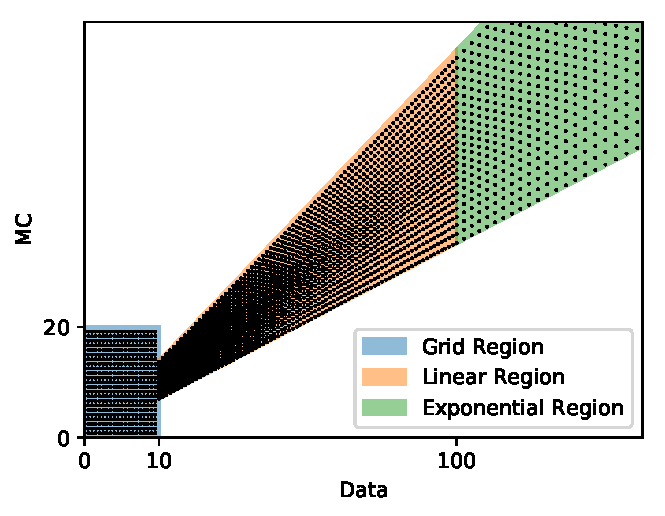
\includegraphics[width=0.7\textwidth]{lut/lut_points}
    \caption{LUT Points}
    \label{fig:lut_points}
\end{figure}

\begin{figure}
    \centering
    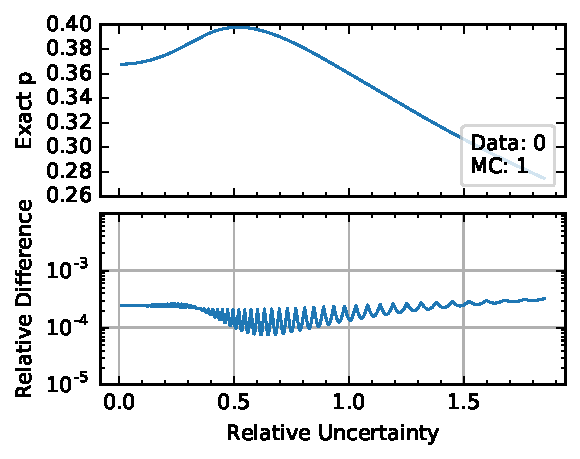
\includegraphics[width=0.49\textwidth]{lut/lut_uncert1}
    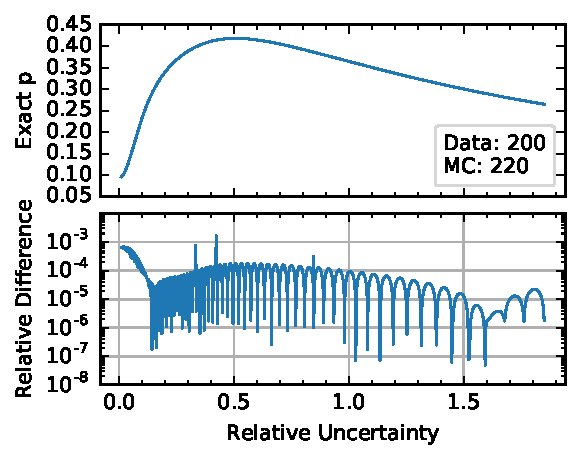
\includegraphics[width=0.49\textwidth]{lut/lut_uncert2}
    \caption{LUT Relative Differences depending on relative uncertainty}
    \label{fig:lut_reldiff_reluncert}
\end{figure}

\begin{figure}
    \centering
    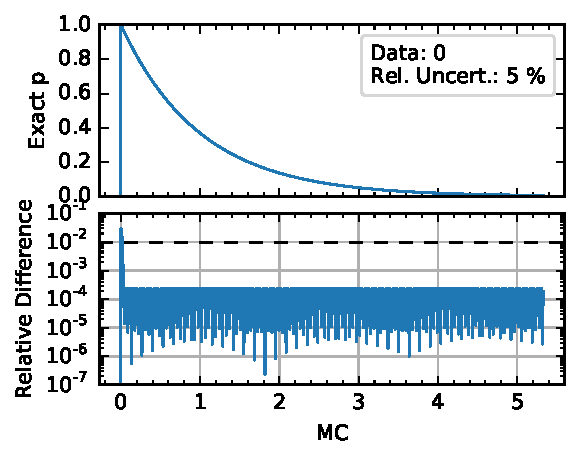
\includegraphics[width=0.49\textwidth]{lut/lut0a}
    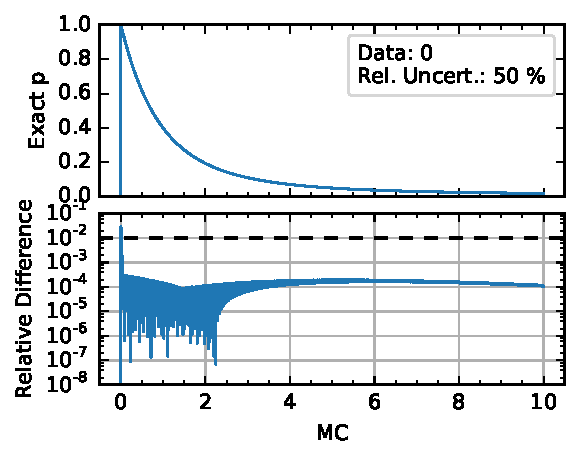
\includegraphics[width=0.49\textwidth]{lut/lut0b}
    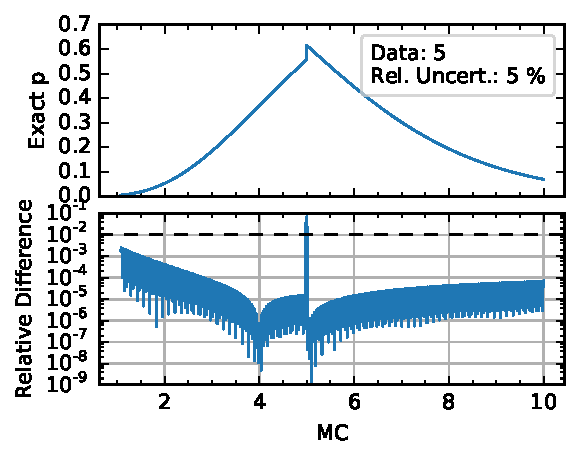
\includegraphics[width=0.49\textwidth]{lut/lut1a}
    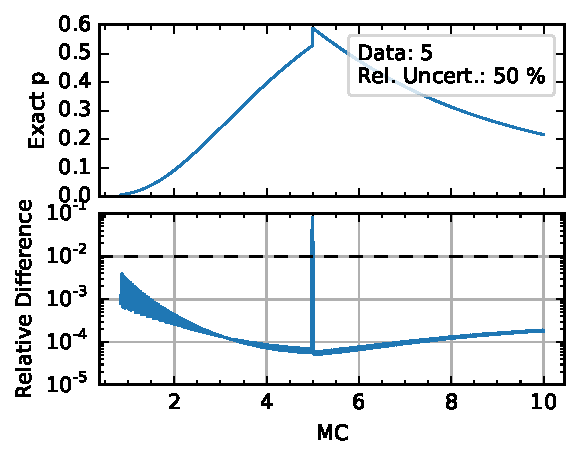
\includegraphics[width=0.49\textwidth]{lut/lut1b}
     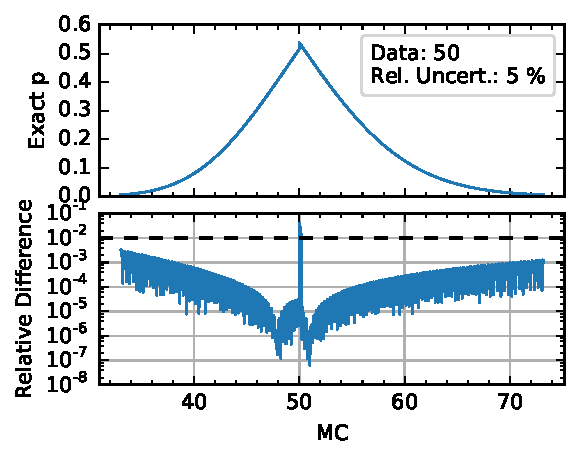
\includegraphics[width=0.49\textwidth]{lut/lut2a}
    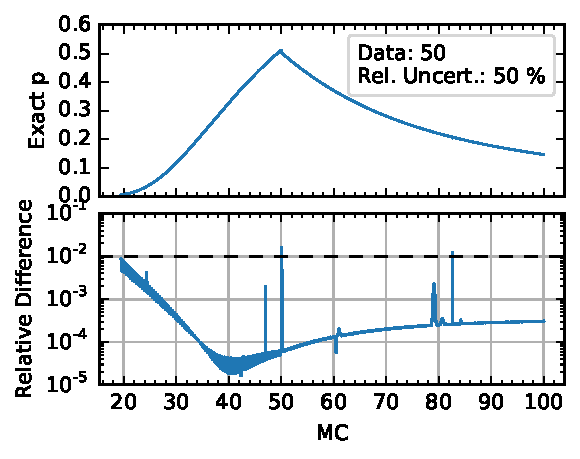
\includegraphics[width=0.49\textwidth]{lut/lut2b}
    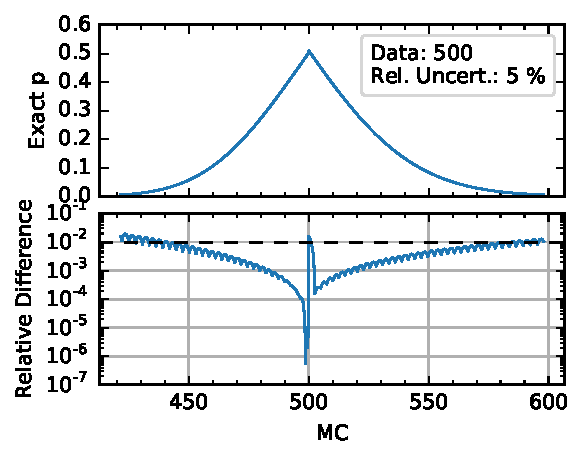
\includegraphics[width=0.49\textwidth]{lut/lut3a}  
    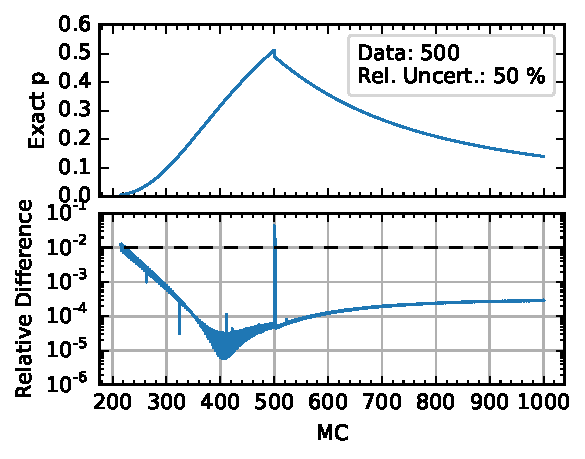
\includegraphics[width=0.49\textwidth]{lut/lut3b}
    \caption{LUT Relative Differences depending on MC (fixed data)}
    \label{fig:lut_reldiff_mc}
\end{figure}

Additionally accessing coverage with lookup table
Same coverage result as for the full p value



\subsection{Automation}
\begin{figure}
    \centering
    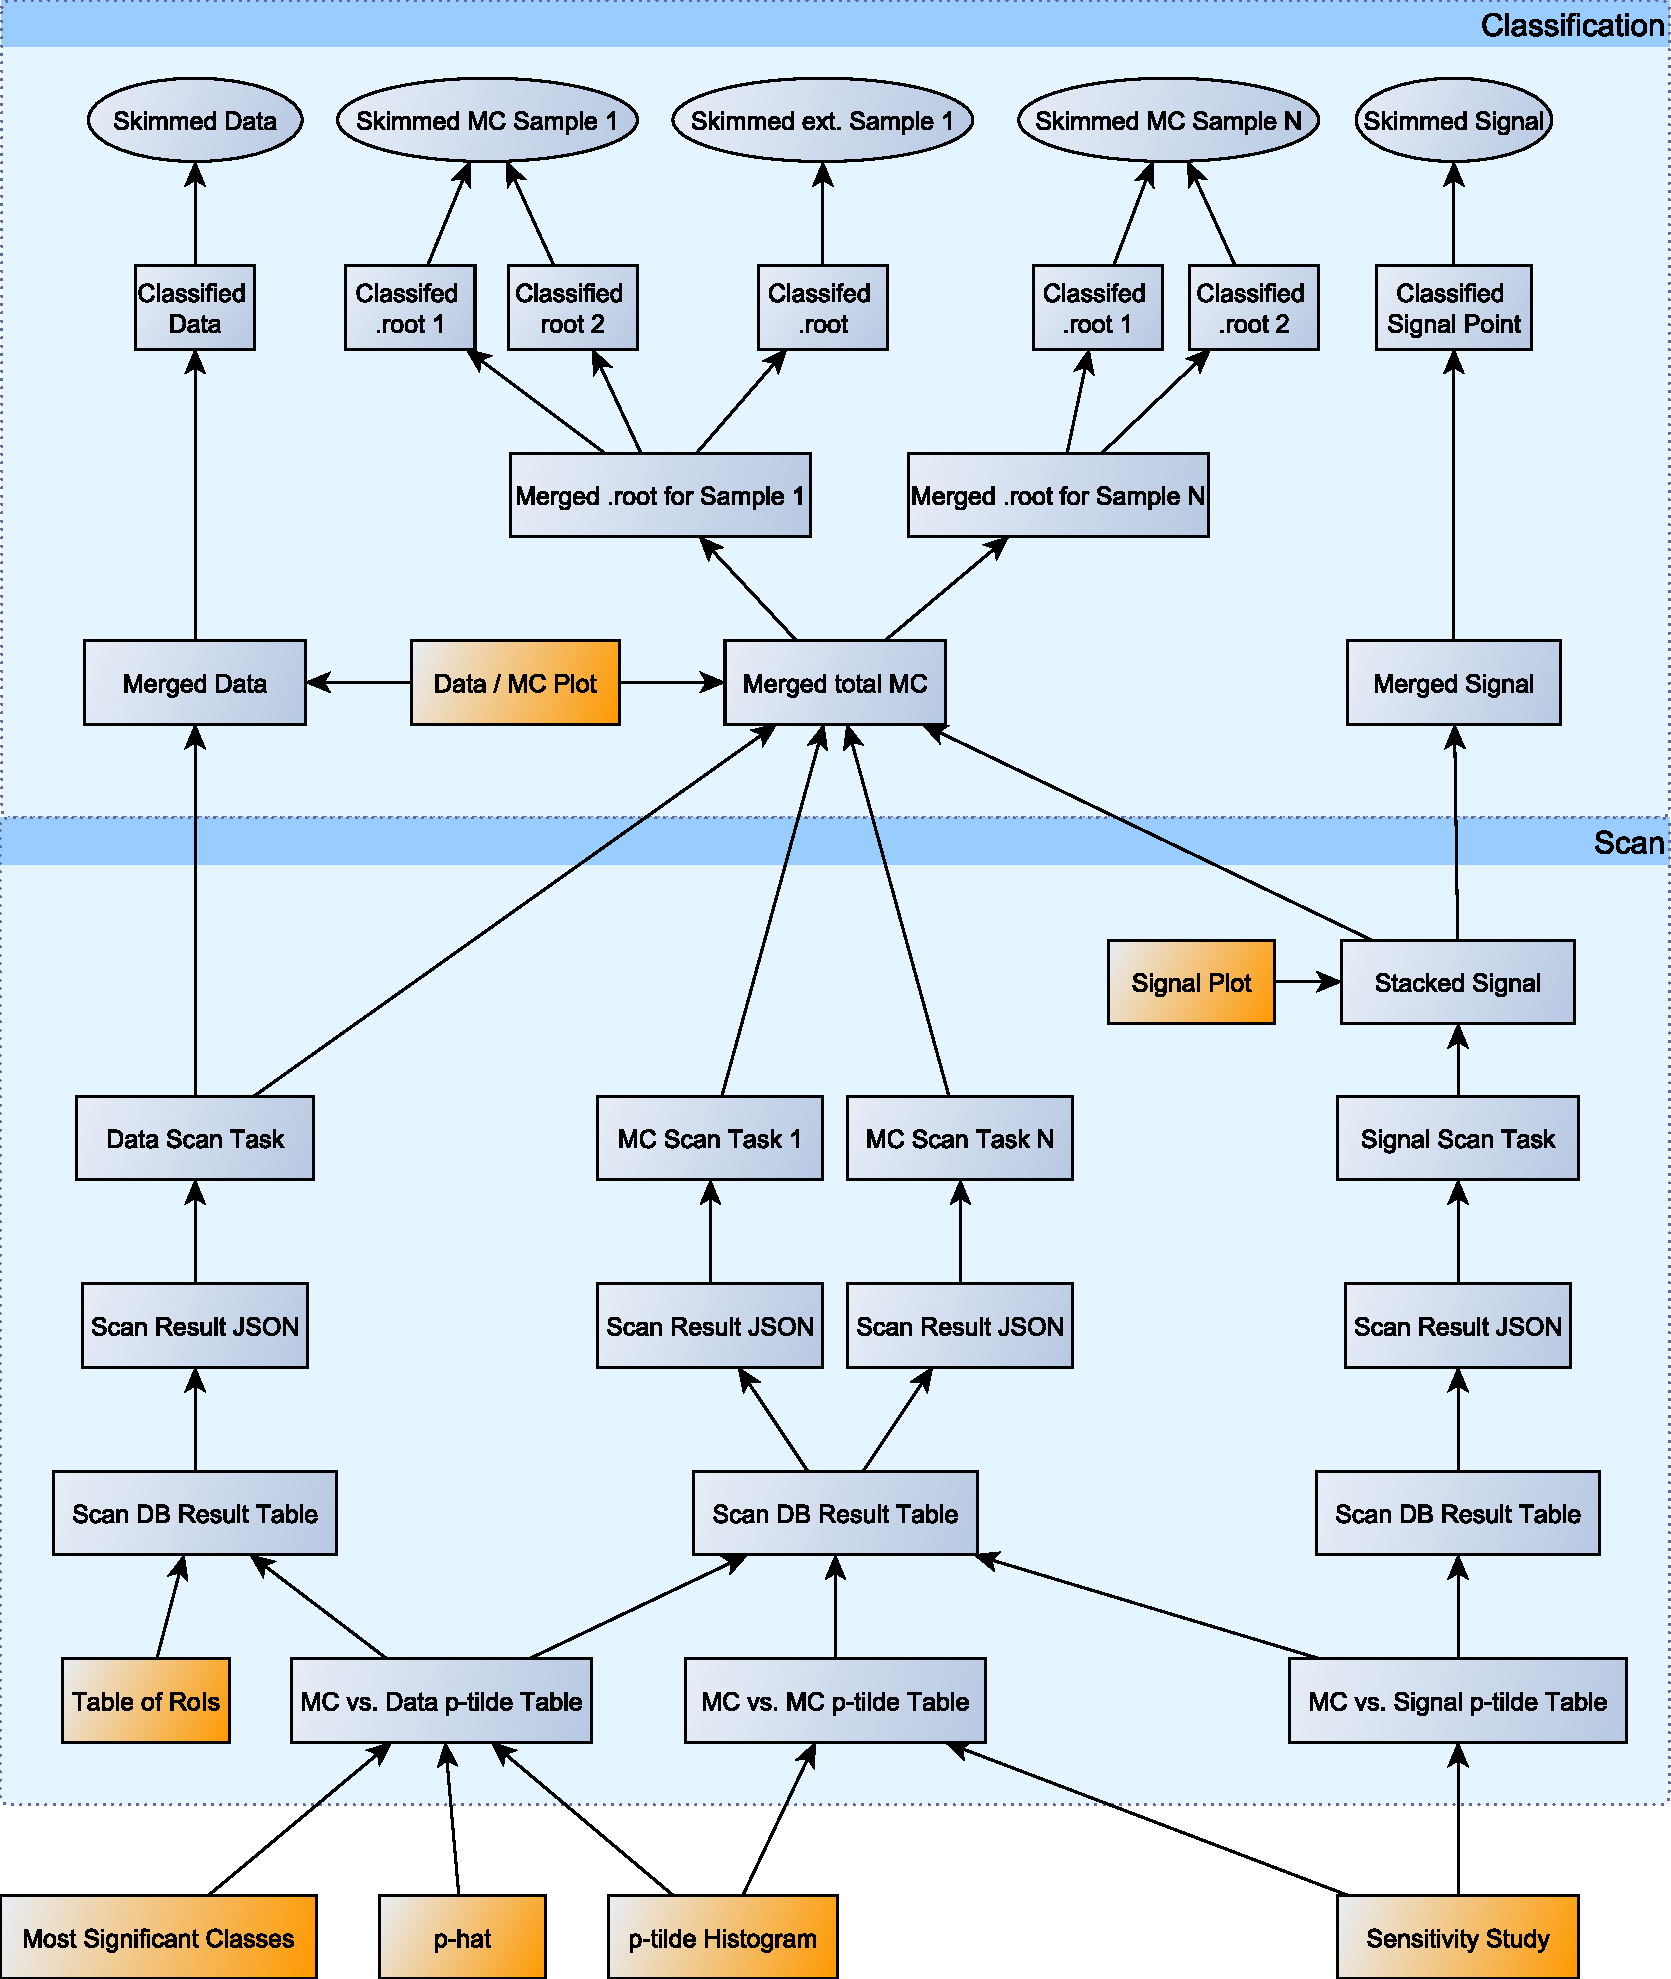
\includegraphics[width=\textwidth]{../music-workflow}
    \vspace{0.5em}
    \caption{Implementation of the MUSiC-Workflow. Using the Luigi-Automation Framework, these steps are performed on demand.}
    \label{fig:music_workflow}
\end{figure}

Luigi

At the time of writing: only classification automated, scan still manually calling scripts